% !TeX root = ../pres.tex

\section{Wellenlänge}
    \begin{myframe}{}
        \begin{figure}
            \centering
            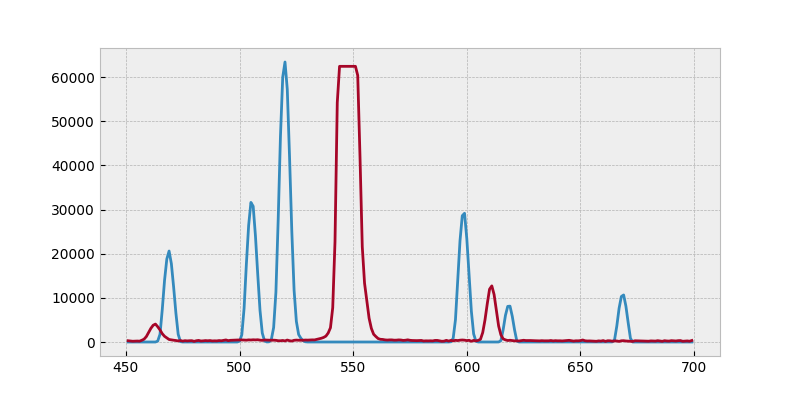
\includegraphics[width=.8\paperwidth]{img/wl.png}
            \caption{Cadmium- (Rot) und Neon- (Blau) Linien (y: Int arbitr\"ar, x: pos in px)}
        \end{figure}
    \end{myframe}

    \begin{myframe}{}
        \begin{figure}
            \centering
            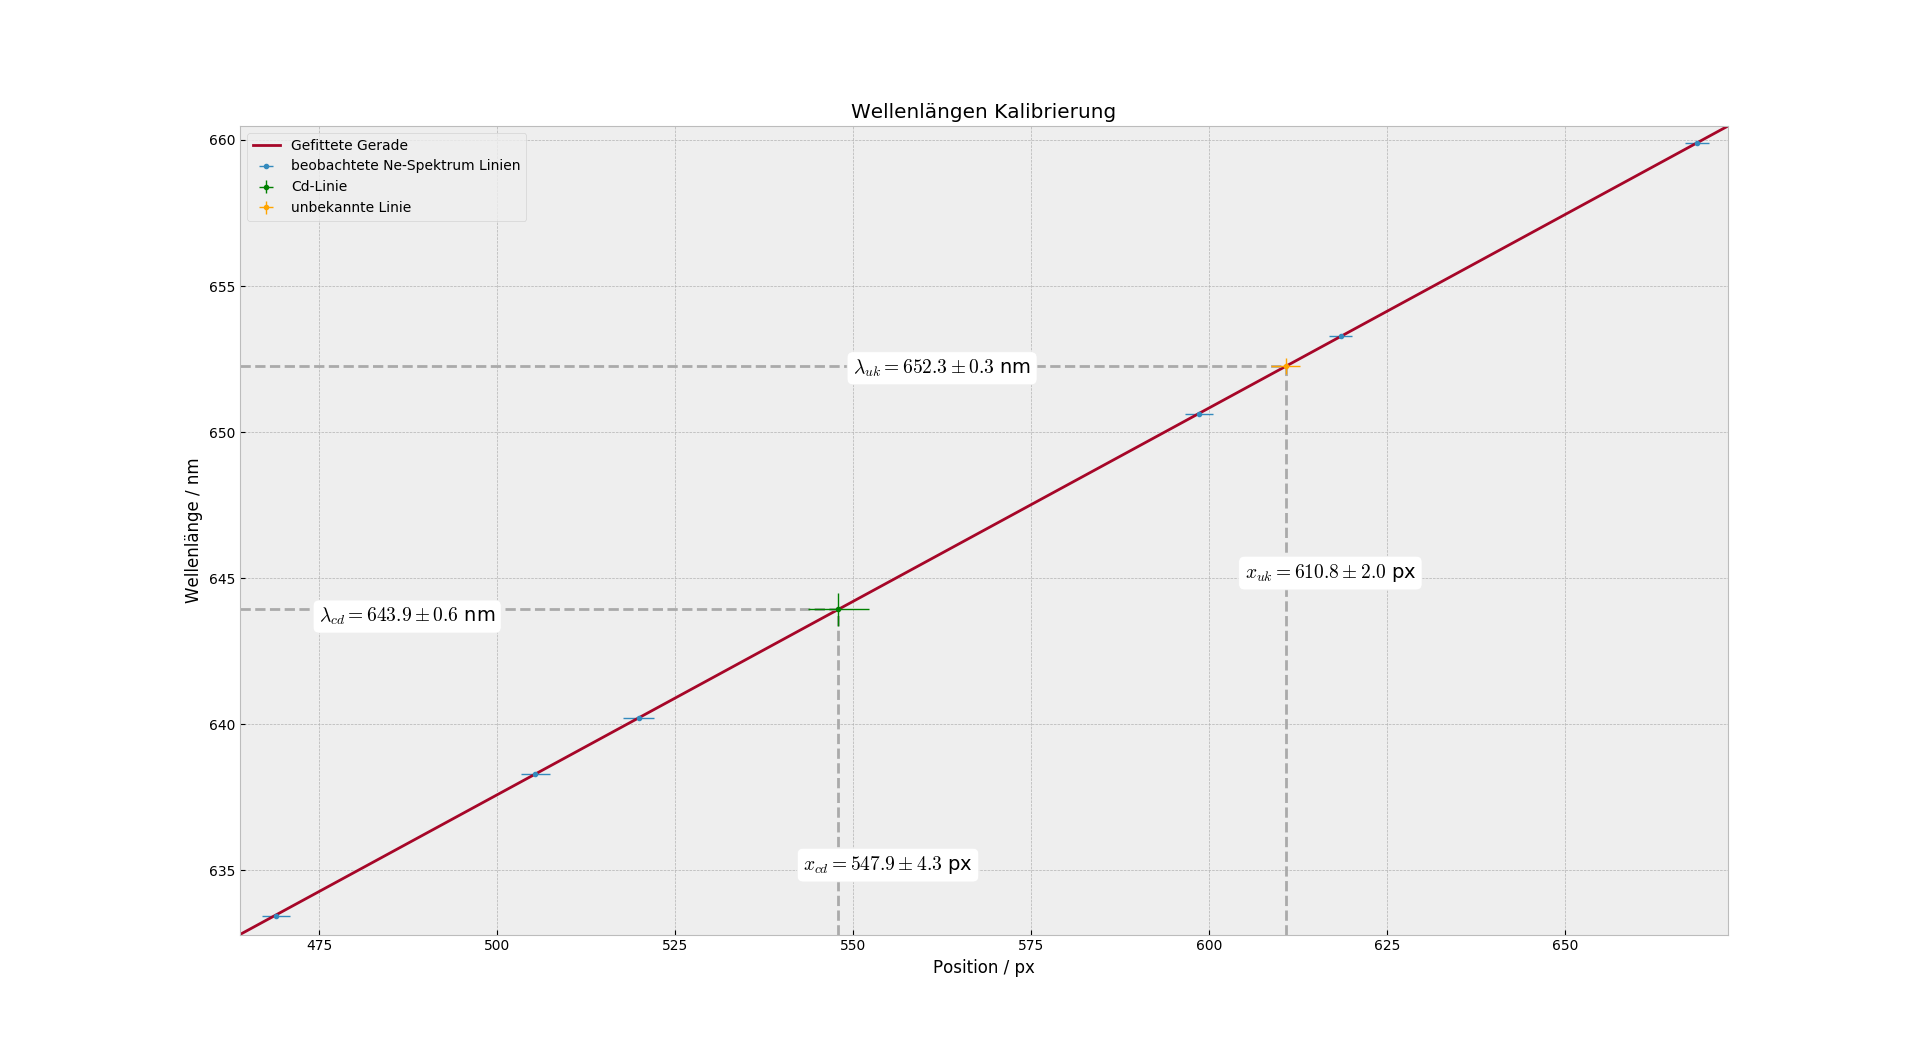
\includegraphics[width=.8\paperwidth]{img/wl_ne_cal}
            \caption{Zusammenhang zwischen Position und Wellenlänge in unseren Beobachtungen}
        \end{figure}
    \end{myframe}

    \subsection{Cadmium-Linie}
        \begin{myframe}{\subsecname}
            \begin{minipage}{.3\textwidth}
                \begin{figure}
                    \centering
                    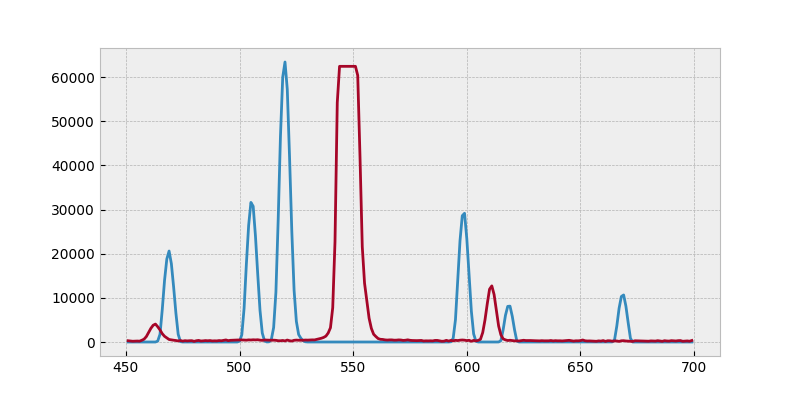
\includegraphics[height=.32\textheight, trim={1.2cm 0 17.5cm 1cm}, clip]{img/wl}
                    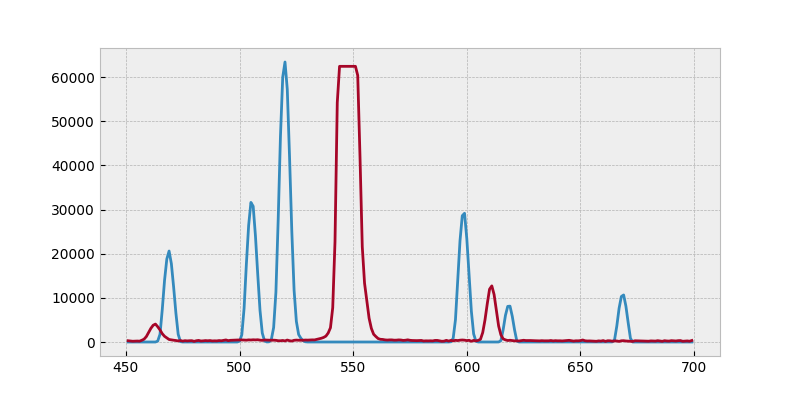
\includegraphics[height=.32\textheight, trim={4cm 0 7cm 1cm}, clip]{img/wl}
                    \caption{Intensit\"atsspektrum, um die Cd-Linie}
                \end{figure}
            \end{minipage}
            \onslide<2->{
                \begin{minipage}{.65\textwidth}
                    \begin{align}
                        a_{Cd} &= \pxCd\\
                        \lambda_{Cd} &= \lambdaCd\\
                        \nonumber\\
                        \lambda_{Cd,theo} &= \lambdaCdTheo\qquad\rightarrow\SI{0.14}{\sigma}
                    \end{align}
                \end{minipage}
            }
        \end{myframe}

    \subsection{unbekannte Linie}
        \begin{myframe}{\subsecname}
            \begin{minipage}{.3\textwidth}
                \begin{figure}
                    \centering
                    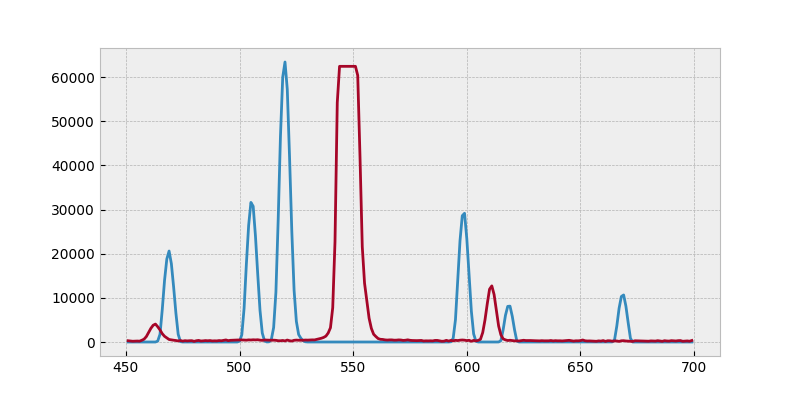
\includegraphics[height=.32\textheight, trim={1.2cm 0 17.5cm 5cm}, clip]{img/wl}
                    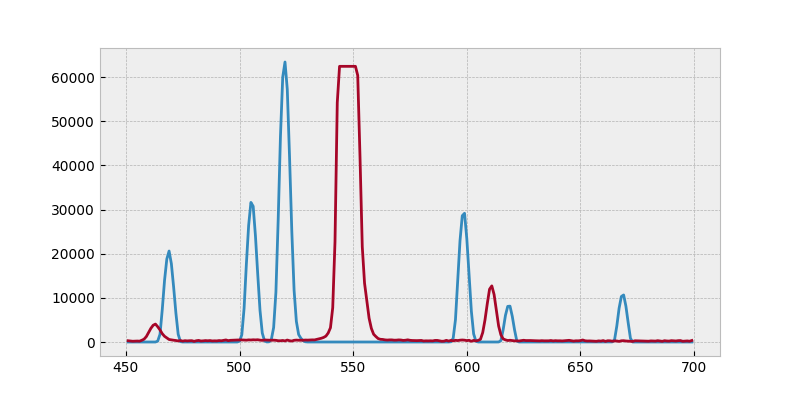
\includegraphics[height=.32\textheight, trim={10cm 0 5cm 5cm}, clip]{img/wl}
                    \caption{Intensit\"atsspektrum, um die unbekannte Linie}
                \end{figure}
            \end{minipage}
            \onslide<2->{
                \begin{minipage}{.65\textwidth}
                    \begin{align}
                        a_{uk} &= \SI{610.8+-4}{px}\\
                        \lambda_{uk} &= \lambdaUk\\
                        \nonumber\\
                        \lambda_{Th\ I} &= \lambdaTh\\
                        \lambda_{Xe\ I} &= \lambdaXe
                    \end{align}
                \end{minipage}
            }
        \end{myframe}
